\begin{figure}[hbtp]
  \centering
  \subfigure{
    \label{fig:community-split--all}
    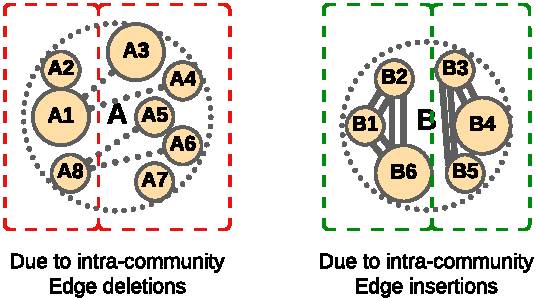
\includegraphics[width=0.80\linewidth]{out/community-split-all.pdf}
  } \\[-1ex]
  \caption{Demonstration of how decreasing or increasing edge density within a community can cause it to split. Here, circles show refined subcommunities, while dotted circles represent the original parent communities from the local-moving phase. Dotted lines indicate edge deletions, double lines represent edge insertions, and brown-filled areas mark regions needing further processing. Red and green boundaries highlight possible split points due to batch updates.}
  \label{fig:community-split}
\end{figure}
